\chapter{Decision Support Systems}

Decision support systems are a type of \textbf{information system}. An information system is an organized collection of resources, people, and procedures finalized to collect, store, process and communicate information needed to support the on-going activities. Information can be represented as images, text, audio, or really any kind of data.

Traditional applications that use databases are called \textbf{OLTP} (\textbf{On Line Transactional Processing}), while decision support applications are called \textbf{OLAP} (\textbf{On Line Analytical Processing}). The key difference between the two is that OLTP systems are used for mostly day-by-day operations, using transactions, while OLAP systems are used to analyze the data to try and extract some hidden knowledge without updating the data. Table \ref{tab:oltp-vs-olap} compares the two in more detail.
\begin{table}[ht]
    \centering
    \small
    \begin{tblr}{
    row{even} = {BrickRed!10},
    columns={130pt, c, m},
    column{1}={75pt}}
    \hline
         & \textbf{OLTP} & \textbf{OLAP} \\
    \hline
    \hline
        \textbf{Function} & Operations & Decisions  \\
        \textbf{Users} & Operatives (clerk, IT professional) & Knowledge workers (managers, analysts) \\
        \textbf{Detail} &  Analytic & May be aggregated \\
        \textbf{Usage} & Repetitive & Ad hoc \\
        \textbf{Data} & Current & Historic \\
        \textbf{Data origin} & Internal & Internal and external \\
        \textbf{Items per operation} & Few (tens) & Many (millions) \\
        \textbf{Updates} & Frequent, small & Rare, massive \\
        \textbf{Stored in} & Database & Data Warehouse/DSS \\
    \hline
    \end{tblr}
    \caption{Comparison between OLTP and OLAP systems.}
    \label{tab:oltp-vs-olap}
\end{table}
While in traditional systems there is usually only a single database containing all the information, in DSS there are multiple data warehouses, one for each analysis.

\section{Data Warehouses}
More formally, a data warehouse can be defined as follows:
\BoxDef{Data warehouse}{
A data warehouse is a subject-oriented, integrated, non-volatile, and time-varying collection of data in support of management's decisions.
}
\begin{itemize}
    \item \textbf{Subject-oriented} means that data is stored by subject, not by applications, unlike traditional databases.
    
    \item \textbf{Integrated} means that data is gathered from a variety of sources and merged.
    
    \item \textbf{Non-volatile} means data is not changed interactively, but may be updated periodically.

    \item \textbf{Time-varying} means that data is assumed to be historical, collected over a long period of time, not necessarily up-to-date, in order to gather knowledge about the operations to be analyzed.
\end{itemize}

\subsection{Architecture}
The term ``data warehousing'' is used to refer to the process of organizing data in a data warehouse to allow end users to analyze it with business intelligence applications. The most common architecture is a three-layer one, composed of the \textbf{data sources}, \textbf{data staging}, and \textbf{data warehouse}.

The data warehouse is loaded with data extracted via \textbf{ETL} (\textbf{Extract, Transform, and Load}) applications from the many different sources of data in the previous layer, bringing them into a consistent form and performing any kind of cleaning needed, and finally storing them into the data staging. The complexity of data staging depends on the quality of the data sources.
\begin{figure}[ht]
    \centering
    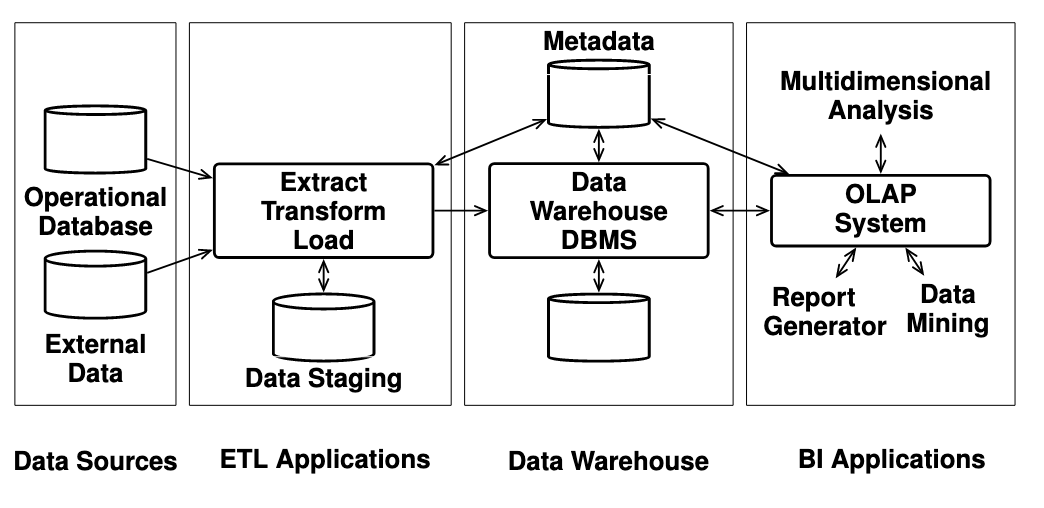
\includegraphics[width=0.5\linewidth]{img/three_layer_architecture.png}
    \caption{Scheme of a data warehouse architecture.}
    \label{fig:enter-label}
\end{figure}

\subsection{Modeling}

The creation of a data warehouse takes place gradually, at different levels of abstraction: it starts with a conceptual model, then a logical model, and finally, a multidimensional cube model.

\subsubsection{Conceptual Model}

The \textbf{Dimensional Fact Model} is a graphical conceptual model for data warehouses. It allows the representation of the following basic information:
\begin{itemize}
    \item \textbf{Facts}: the most important abstraction mechanism is the collection of facts, which are the observations of the performance of a business process. They are usually transactions or events (e.g., sales, clicks, complaints, visits), and may be \textbf{periodic} (one fact for a group of transactions made over a period of time), or \textbf{accumulating} (one fact for the entire life of the event, evolving over time).
    
    Facts are modeled by \textbf{fact tables}, each of which is a rectangle divided in two parts, one containing the fact name, and the other containing the measures.
    
    \item \textbf{Measures}: measures are quantitative information whose aggregation is of interest. The aggregation function is often the sum, but may also be a count, average, max, min, and so on.

    Measures are specified inside the fact tables.
    
    \item \textbf{Dimensions}: dimensions give facts a context: they explain ``who, what, why, when, where'' a fact is happening. A dimension can be described as a set of attributes used to qualify, categorize, or summarize facts in reports.

    Dimensions are represented by a circle connected to the fact table with a straight line, and one additional circle for each attribute of that dimension.
\end{itemize}
In the presence of dimensions, an hierarchical relationship can be modeled among them. For example, imagine a fact table with dimensions relating to dates (Year, Quarter, Month, Week, Day). A hierarchy can be constructed (Day $\rightarrow$ Week $\rightarrow$ Month $\rightarrow$ Quarter $\rightarrow$ Year) such that each element is more general than those coming before it, and less general than those after. In this case, Month is more general than Day, but is less general than Quarter. Formally, each arc of the hierarchy models a \textbf{functional dependency} between the two attributes. Graphically, hierarchies are represented as a directed tree, rooted in a dimension, and with the leaves representing the most general dimensions.

The presence of a hierarchy increases the possibilities of data analysis from different perspectives (so-called multidimensional analysis). If we already analyzed sales by year, we can also analyze them at a deeper level, considering months or days.
\begin{figure}[ht]
    \centering
    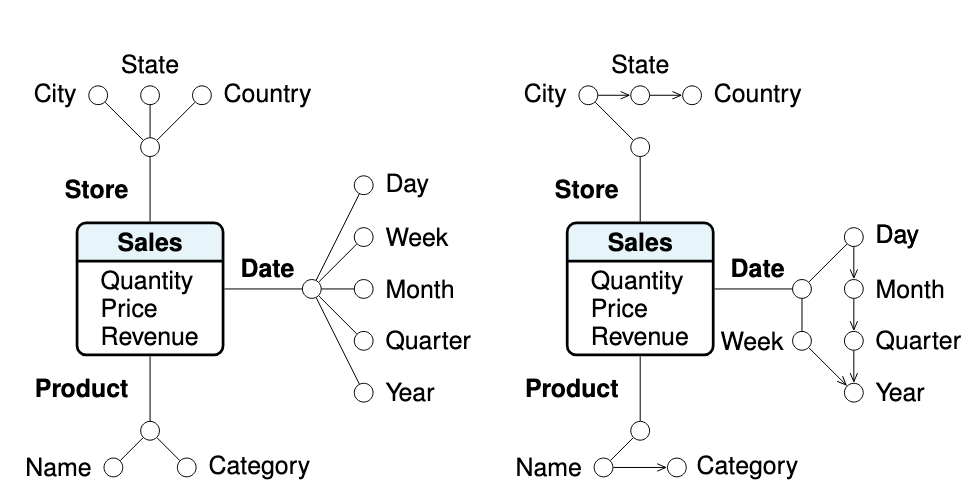
\includegraphics[width=0.75\linewidth]{img/hierarchies.png}
    \caption{Conceptual design without and with hierarchies.}
    \label{fig:hierarchies}
\end{figure}

\subsubsection{Relational Model}

A conceptual model can be transformed into a relational schema by applying a set of mapping rules. The most common schemas are the star schema, the snowflake schema, and the constellation schema.

In a \textbf{star schema}, the fact table is placed a the center, and a foreign key is added for each dimension. Dimensions are also transformed into tables (simply adding all the attributes, without considering hierarchies), and connected to the fact table with a one-to-many relationship.

A \textbf{snowflake schema} is similar to a star schema, but some dimension tables are also normalized, splitting the data into additional tables.

A \textbf{constellation schema} has multiple fact tables that share dimension tables.

\begin{figure}[ht]
    \centering
    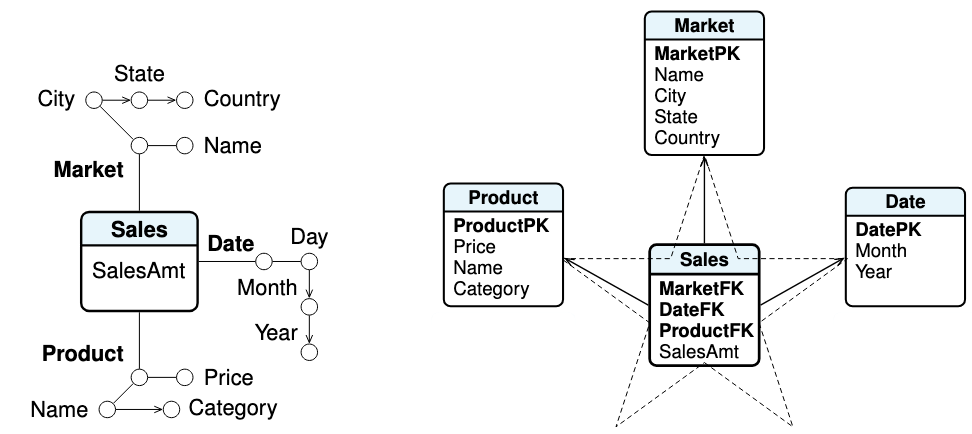
\includegraphics[width=0.65\linewidth]{img/star_schema.png}
    \caption{Star schema.}
    \label{fig:star-schema}
\end{figure} 
\begin{figure}[ht]
    \centering
    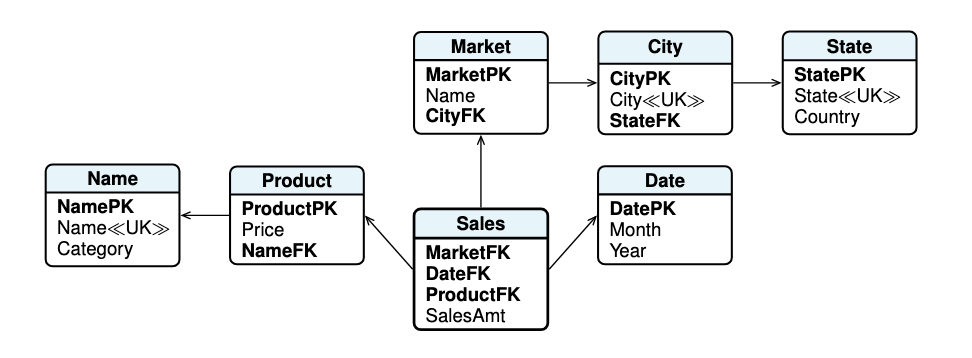
\includegraphics[width=0.65\linewidth]{img/snowflake_schema.png}
    \caption{Snowflake schema.}
    \label{fig:snowflake-schema}
\end{figure}
\begin{figure}[H]
    \centering
    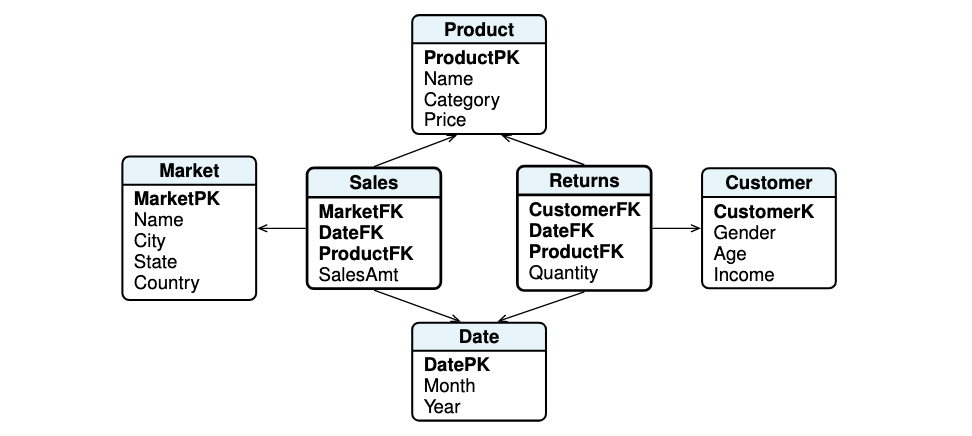
\includegraphics[width=0.65\linewidth]{img/constellation_schema.png}
    \caption{Constellation schema.}
    \label{fig:constellation-schema}
\end{figure}

\subsubsection{Multidimensional Cube Model}

A \textbf{multidimensional data model} (data cube) represents facts with $n$ dimensions as points in an $n$-dimensional space. A point (fact) is identified by the values of its dimensions, and has an associated set of measures. This view is an intuitive way to think about OLAP queries and their results.

For example, imagine a fact table with information about store sales. Each record in the original data has three attributes: a store id, a product id, and an associated quantity. We can see this data as 2-dimensional: the two dimensions are the store and the product id, while the measure is the quantity.
\begin{figure}[ht]
    \centering
    \begin{minipage}{0.49\textwidth}
        \centering
        \begin{tblr}{
            row{even} = {BrickRed!10}
        }
        \hline
           \textbf{StoreId}  & \textbf{ProductId} & \textbf{Qty} \\
        \hline
        \hline
            S1 & P1 & 300 \\
            S2 & P1 & 500 \\
            S3 & P1 & 50 \\
            S1 & P2 & 300 \\
            S2 & P2 & 10 \\
            S3 & P2 & 30 \\
            S1 & P3 & 40 \\
            S3 & P3 & 20 \\
        \hline
        \end{tblr}
        \caption{Fact table.}
    \end{minipage}
    \hfill
    \begin{minipage}{0.49\textwidth}
        \centering
        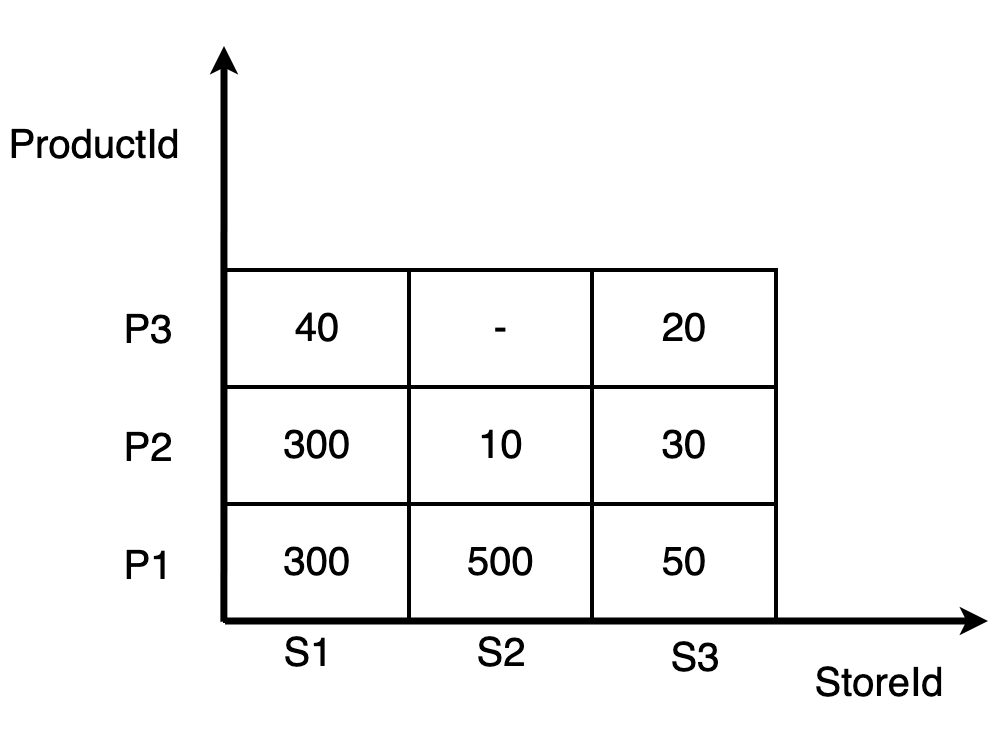
\includegraphics[width=\linewidth]{img/datacube.png}
        \caption{Example data cube.}
    \end{minipage}
\end{figure}
Obviously, this is a very simple case. In real applications, the number of dimensions can be higher than 2 or 3, so the data cube cannot be visualized in its entirety. These cubes can be manipulated via a specific geometric language, of which we can define these basic operations:
\begin{itemize}
    \item \textbf{Slice}: slicing means ``cutting'' the cube by selecting on a specific value for one dimension.

    \item \textbf{Dice}: dicing is similar to slicing, but selects on two or more dimensions.

    \item \textbf{Pivot}: pivoting performs a rotation of the data axes, providing an alternative presentation of the data.

    \item \textbf{Roll-up}: rolling-up compresses the cube across a dimension, summarizing the information provided bu that dimension. It can be seen as similar to a GroupBy done on all other dimensions not involved in the roll-up.

    \item \textbf{Drill-down}: it is the reverse of roll-up. It produces more detailed data across a dimension.
\end{itemize}

Assume that, given a data cube, eacj dimension is extended with an additional value, ``*'', representing summarization along that dimension. Then, the cube can be extended with borders containing the values of the sum along each possible combination of dimensions. When we select a subcube by specifying a dimension instead of its value (e.g., (StoreId, *)), we get a roll-up of the original data across all other dimensions, called \textbf{cuboid}.

An order relation can be defined between cuboids: $C1 \preceq C2$ if $C1$ can be computed from $C2$. This order is visualized using a \textbf{data warehouse lattice}. In the example below, we can see how the cuboid (StoreId) can be computer from (StoreId, ProductId), but (StoreId, ProductId, DateId) cannot be computed from (StoreId, ProductId). So, how do we choose which of these cuboids to store? Obviously, the source data allows us to compute all other cuboids. However, if the queries most commonly executed only consider a subset of the dimensions, we may store those (or store one of those above them).

\begin{figure}[ht]
    \centering
    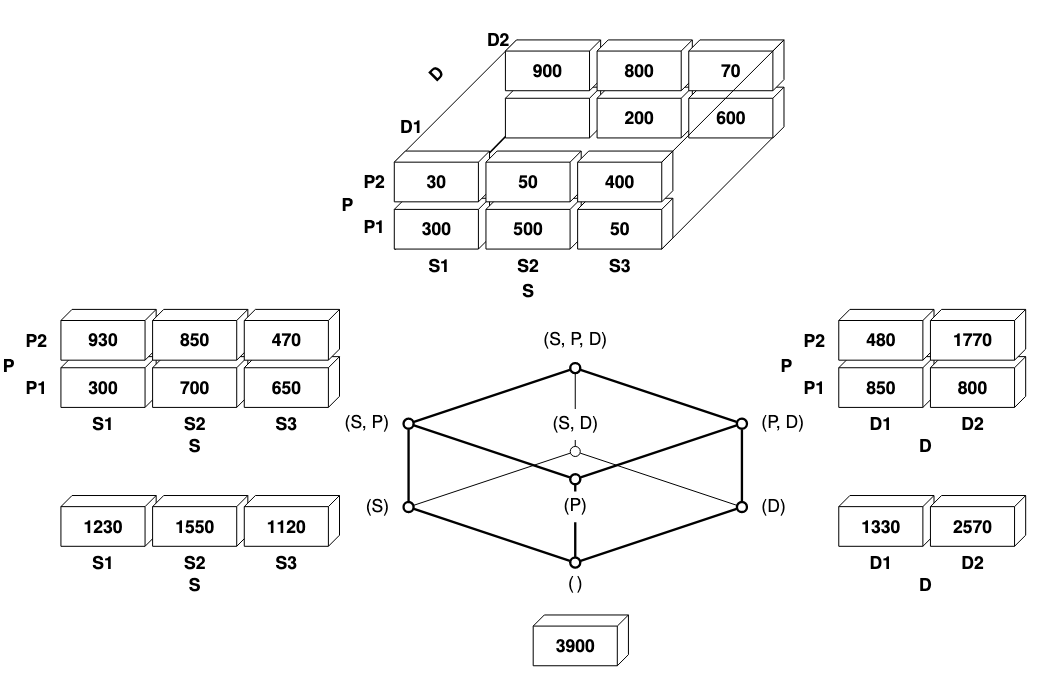
\includegraphics[width=0.8\linewidth]{img/lattice.png}
    \caption{A data warehouse lattice. The data cube it corresponds to has three dimensions: StoreId, ProductId, and Date.}
    \label{fig:lattice}
\end{figure}